\documentclass[conference]{IEEEtran}
\IEEEoverridecommandlockouts
\usepackage{cite}
\usepackage{amsmath,amssymb,amsfonts}
\usepackage{algorithm}
\usepackage{algorithmic}
\usepackage{graphicx}
\usepackage{textcomp}
\usepackage{xcolor}
\usepackage{url}
\usepackage{booktabs}
\usepackage{balance}

% Tell LaTeX to search 'Figures/', 'figures/', and the root directory for uploaded images
\graphicspath{{Figures/}{figures/}{./}}

\def\BibTeX{{\rm B\kern-.05em{\sc i\kern-.025em b}\kern-.08em T\kern-.1667em\lower.7ex\hbox{E}\kern-.125emX}}
\begin{document}

\title{CapDrift-FL: Capability- and Drift-Aware Federated Learning for Heterogeneous Edge AI Systems}

\author{\IEEEauthorblockN{William Ileka}
\IEEEauthorblockA{School of Computing\\
DePaul University\\
Chicago, IL, USA\\
wileka@depaul.edu}
\and
\IEEEauthorblockN{Brendan Kechtban}
\IEEEauthorblockA{School of Computing\\
DePaul University\\
Chicago, IL, USA\\
bkechtba@depaul.edu}}

\maketitle

\begin{abstract}
Federated learning (FL) enables distributed artificial intelligence across edge systems without centralizing private local data. However, heterogeneous edge nodes exhibit disparate processing capabilities, while data that are not independent and identically distributed (non-IID) can cause extended local computation to intensify client drift. Uniform local training underutilizes fast nodes, whereas capability-driven training can destabilize global learning. This paper proposes CapDrift-FL, a synchronous FL framework that coordinates runtime capability estimation, mandatory minimum local workloads, directional drift gating on surplus computation, and contribution-bounded aggregation. In five-client physical edge-cluster evaluations on Cisco UCS servers, CapDrift-FL reduces round idle waiting by 69.1\% (from 3.41\,s to 1.05\,s) and increases execution-time utilization to 98.2\% relative to uniform training, while highlighting early-round accuracy tradeoffs from deeper local updates. In controlled eight-round non-IID simulations ($\alpha = 0.5$), the framework achieves 88.89\% validation accuracy in component ablation and completes training in 73.3\,s compared to 126.1\,s for FedNova (a 41.8\% runtime reduction). Under extreme skew ($\alpha = 0.1$), directional drift gating halts 20 divergent surplus blocks across five evaluation rounds, preserving a 3.27 percentage point validation advantage over FedAvg.
\end{abstract}

\begin{IEEEkeywords}
Client drift, edge artificial intelligence, federated learning, heterogeneous computing, non-IID data, straggler mitigation.
\end{IEEEkeywords}

\section{Introduction}\label{sec:intro}
Federated learning (FL) \cite{mcmahan2017} enables distributed artificial intelligence models to be trained across edge devices without transferring raw local data to a central repository. This paradigm is especially advantageous in edge systems where data locality, privacy regulations, and bandwidth limitations preclude centralizing sensor or diagnostic records. However, heterogeneous edge platforms introduce substantial disparities in processing capability, memory bandwidth, and communication latency among participating nodes \cite{chai2020tifl,lai2021oort,wong2026edge}.

In conventional synchronous FL, the coordinator assigns an identical local training workload to participating nodes and completes a communication round only after receiving all updates. Slower stragglers delay round completion, forcing faster nodes to remain idle at the synchronization barrier and underutilizing available hardware capacity. Capability-aware scheduling addresses this inefficiency by assigning additional local optimization steps to faster nodes in proportion to their processing speeds \cite{shin2022fedbalancer,li2024fedcompass,narmadha2025fedeff}.

Nevertheless, capability-driven training introduces a severe statistical challenge when local datasets are not independent and identically distributed (non-IID). When a high-throughput node performs extensive local gradient descent over its skewed partition, its parameter trajectory moves progressively farther from global consensus. As a consequence, additional local computation can improve systems-level hardware utilization while simultaneously aggravating client drift. Furthermore, updates produced by extended local computation can exert disproportionate influence during server aggregation. Local training on heterogeneous edge nodes must therefore be regulated according to executable computational speed, evolving statistical trajectory, and aggregation influence.

Existing methods address subsets of these challenges. FedProx stabilizes local optimization through a proximal regularization penalty \cite{li2020fedprox}, SCAFFOLD applies control variates to correct drift \cite{karimireddy2020scaffold}, and FedNova normalizes local updates during server aggregation to eliminate objective inconsistency \cite{wang2020fednova}. Adaptive Local Training regulates local steps based on local--global gradient alignment \cite{shenaj2025alt}, while FedCompass schedules client workloads according to computing power \cite{li2024fedcompass}. However, runtime capability adaptation, surplus-computation drift gating, and aggregation influence control remain fragmented across separate paradigms.

To address these coupled challenges, this paper proposes CapDrift-FL, a synchronous federated edge learning framework that coordinates four interlinked mechanisms: (i) runtime capability estimation based on measured local training throughput, (ii) mandatory minimum local training across all participating nodes, (iii) block-wise directional drift gating applied strictly to surplus computation, and (iv) contribution-bounded server aggregation to limit excessive parameter influence.

The proposed framework is evaluated through physical edge-cluster experiments and controlled federated-learning simulations involving heterogeneous client capabilities and non-IID data distributions. Comparisons with established FL baselines examine model accuracy, training duration, synchronization waiting, and scalability. The results illustrate the accuracy--efficiency tradeoffs associated with capability-aware training and drift control.

The remainder of the paper is organized as follows. Section~\ref{sec:related} reviews related work. Section~\ref{sec:model} presents the system model and federated learning formulation. Section~\ref{sec:framework} details the proposed CapDrift-FL framework. Section~\ref{sec:eval} provides performance evaluations across physical and controlled environments. Finally, Section~\ref{sec:conclusion} concludes the paper, followed by data availability and references.

\section{Related Work}\label{sec:related}
Resource-aware federated learning methods focus on mitigating straggler effects and managing heterogeneous client resources. TiFL groups clients into distinct resource tiers to minimize round latency \cite{chai2020tifl}. Oort guides client selection based on statistical utility and system execution speed \cite{lai2021oort}, while FedBalancer dynamically adjusts local sample batches and deadlines to balance progress \cite{shin2022fedbalancer}. Further studies adapt local client selection and aggregation schemes under edge resource constraints \cite{zhang2022adaptive,hou2024atafl}. Fan et~al.~\cite{fan2026fedcer} formulate joint client selection and epoch allocation for heterogeneity-aware FL in resource-constrained edge environments, and Liu et~al.~\cite{liu2024fedsc} design adaptive clustering to reduce straggler waiting across wireless edge networks. Wong et~al.~\cite{wong2026edge} empirically analyze resource allocation bottlenecks across edge and IoT platforms. Although these methods improve systems-level throughput or client participation, they primarily regulate scheduling, resource tiers, or selection policies rather than actively monitoring the statistical trajectory of extended local computation during training.

Capability-aware workload assignment allocates local work according to processing speed. FedCompass employs a computing-power-aware scheduler to assign heterogeneous local step budgets and reduce synchronization waiting \cite{li2024fedcompass}. FedEff similarly optimizes local epoch allocation according to client computation and transmission speeds \cite{narmadha2025fedeff}. These approaches demonstrate clear systems benefits in reducing barrier idle waste. However, under non-IID label skew, allocating unconstrained local computation to faster nodes can accelerate statistical divergence toward private local optima.

A complementary body of literature investigates statistical heterogeneity and client drift. FedProx incorporates a proximal term into the local objective to constrain updates near the global model \cite{li2020fedprox}. SCAFFOLD uses client and server control variates to estimate and correct gradient drift directions \cite{karimireddy2020scaffold}. FedNova addresses objective inconsistency by scaling client updates by their executed step counts during server aggregation \cite{wang2020fednova}. Adaptive Local Training adjusts local work based on local--global gradient similarity \cite{shenaj2025alt}. Nevertheless, these methods do not separate an edge node's executable runtime capability ceiling from the decision to terminate computation once a mandatory minimum workload has been satisfied.

Aggregation control mechanisms restrict update magnitude and influence. FedLAGC integrates layer-adaptive submodel extraction with gradient correction to handle system heterogeneity \cite{hu2026fedlagc}, while adaptive contribution clipping bounds update norms during federated optimization \cite{andrew2021clipping}. These aggregation mechanisms constrain submitted update magnitudes, yet they operate retrospectively at the coordinator and cannot prevent clients from performing statistically unaligned surplus computation prior to transmission.

CapDrift-FL bridges the gap between exploiting heterogeneous edge processing capacity and regulating the learning effect of additional local training. The framework coordinates runtime capability budgeting, mandatory baseline workloads, block-wise directional drift gating on surplus blocks, and contribution-bounded aggregation.

\section{System Model}\label{sec:model}

\subsection{Federated Edge AI Architecture}\label{subsec:architecture}
The federated edge AI system consists of a logically centralized coordinator workstation and a set $N$ of $|N|$ distributed edge nodes. Each edge node $i \in N$ holds a private local dataset $D_i$ containing $n_i = |D_i|$ training samples, with total dataset size $n = \sum_{i \in N} n_i$. Raw local data remain strictly confined to the originating edge node throughout the training process. 

At the start of communication round $t$, the coordinator determines the participating client cohort $\mathcal{C}_t \subseteq N$ and broadcasts the current global model parameter vector $w^{(t-1)}$. In the nominal deployments evaluated in this paper, all available clients participate in each round ($|\mathcal{C}_t| = |N|$), while the framework remains compatible with partial client selection policies. Upon receiving $w^{(t-1)}$, each participating client executes local optimization, measures its effective training throughput, and transmits its model parameter displacement $\Delta_i(t)$ and throughput observation $q_i(t)$ back to the coordinator over the communication fabric.

\begin{figure}[t]
\centering
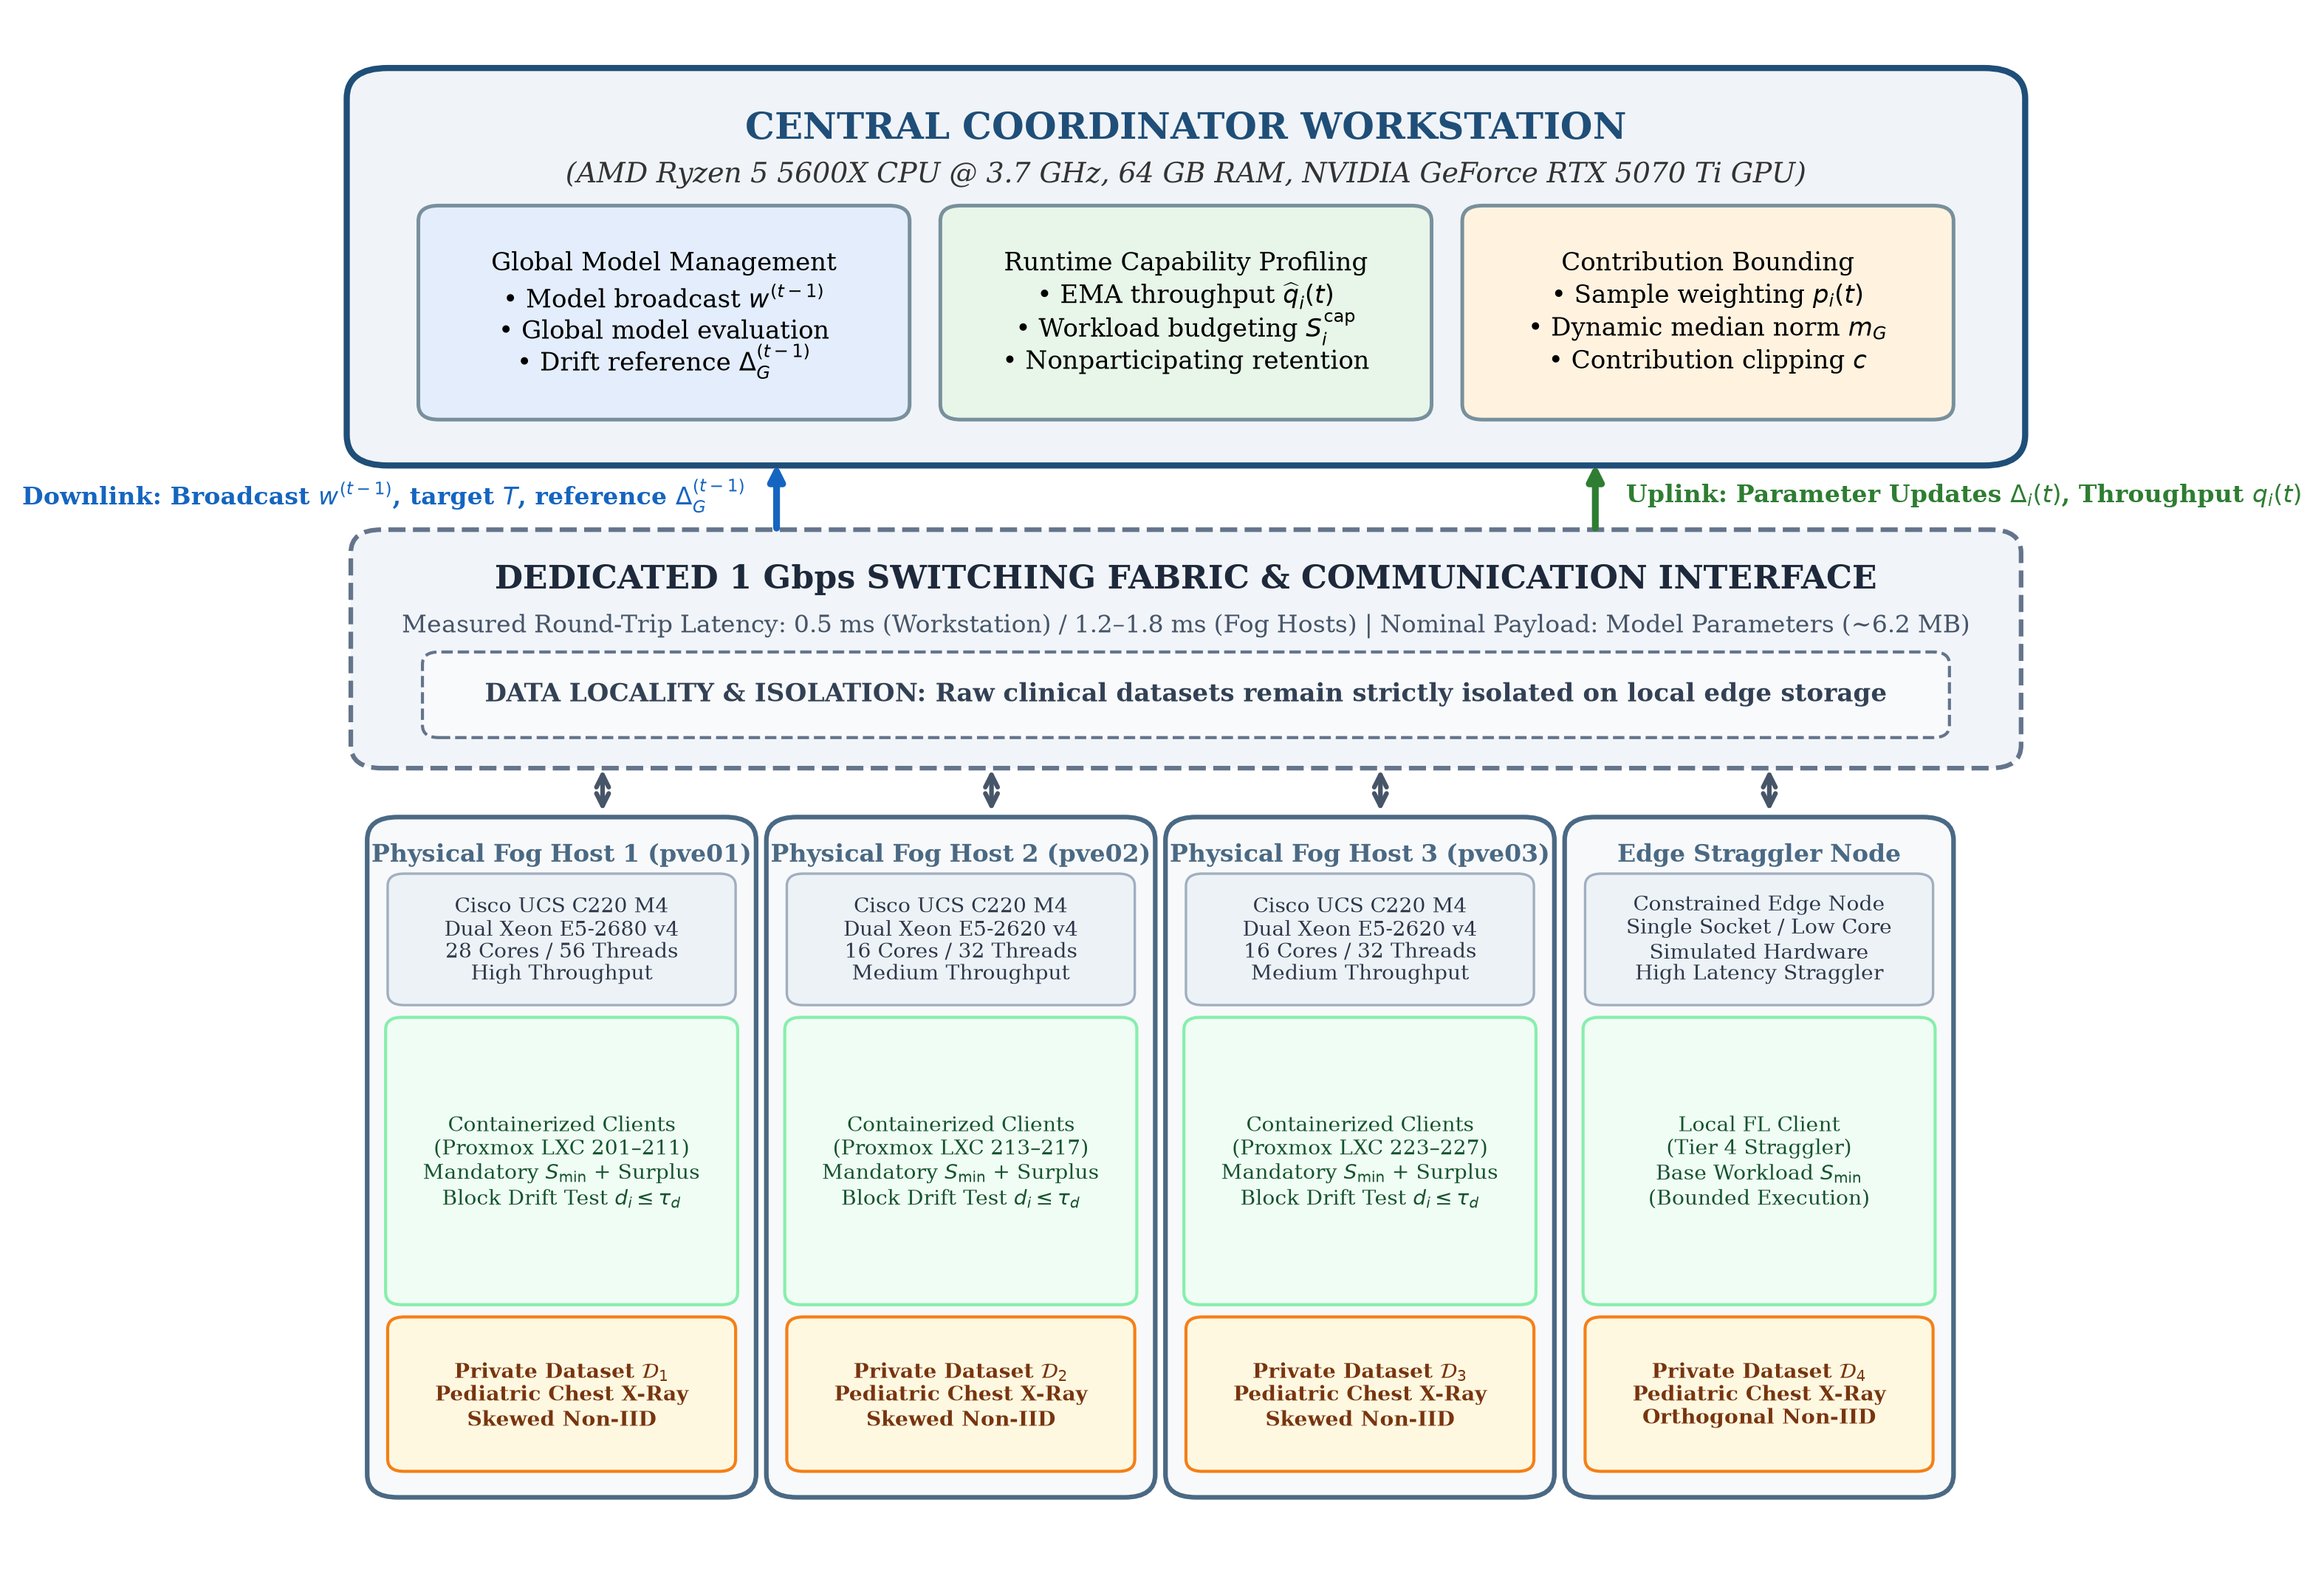
\includegraphics[width=\columnwidth]{fig_system_architecture.png}
\caption{CapDrift-FL federated edge AI system architecture, illustrating central coordinator orchestration, 1\,Gbps communication fabric with local data isolation, and heterogeneous edge hosts running containerized FL clients on private local datasets.}
\label{fig:arch}
\end{figure}

\subsection{Federated Learning Model}\label{subsec:learning}
Let $w \in \mathbb{R}^d$ represent the global model parameters and $\ell(w, z)$ denote the loss computed on sample $z$. Each client $i \in N$ defines its local objective function as $F_i(w) = n_i^{-1} \sum_{z \in D_i} \ell(w, z)$. The canonical federated optimization objective is
\begin{equation}
\min_{w \in \mathbb{R}^d} F(w) = \sum_{i \in N} \frac{n_i}{n} F_i(w).
\label{eq:objective}
\end{equation}
Equation~(\ref{eq:objective}) represents the underlying sample-weighted optimization problem, whereas CapDrift-FL modifies client-side local workload execution and coordinator-side model aggregation.

At the beginning of round $t$, each participating client initializes its local parameter vector as $w_{i,0}^{(t)} = w^{(t-1)}$ and local velocity vector as $v_{i,0}^{(t)} = 0$. Local optimization is performed using stochastic gradient descent (SGD) with momentum according to
\begin{align}
v_{i,s+1}^{(t)} &= \mu v_{i,s}^{(t)} + g_i\!\left(w_{i,s}^{(t)}, \xi_{i,s}^{(t)}\right), \label{eq:velocity} \\
w_{i,s+1}^{(t)} &= w_{i,s}^{(t)} - \eta_l v_{i,s+1}^{(t)}, \label{eq:localsgd}
\end{align}
where $\mu \in [0, 1)$ denotes the momentum coefficient ($\mu = 0.9$ in our implementation), $\eta_l > 0$ is the local learning rate, $\xi_{i,s}^{(t)}$ is a mini-batch of training samples drawn from $D_i$ at local step $s$, and $g_i(w_{i,s}^{(t)}, \xi_{i,s}^{(t)})$ is the stochastic gradient including weight decay regularization. Each client completes $S_i(t)$ local SGD steps executed in control blocks of size $K$. The final model parameter displacement returned by client $i$ is $\Delta_i(t) = w_i^{(t)} - w^{(t-1)}$.

\subsection{Client Capability and Model Drift}\label{subsec:state}
Client processing throughput serves as the runtime capability signal. During round $t$, client $i$ completes $S_i(t)$ local steps over active training duration $\tau_i^{\mathrm{tr}}(t) > 0$, yielding measured throughput
\begin{equation}
q_i(t) = \frac{S_i(t)}{\tau_i^{\mathrm{tr}}(t)},
\label{eq:throughput}
\end{equation}
measured in completed local SGD steps per second ($\text{steps/s}$). The training interval $\tau_i^{\mathrm{tr}}(t)$ encompasses local mini-batch optimization and drift assessment, excluding network transmission and server aggregation.

To mitigate sensitivity to transient hardware fluctuations, the coordinator updates a smoothed capability estimate via exponential moving average:
\begin{equation}
\widehat q_i(t+1) = \beta \widehat q_i(t) + (1 - \beta) q_i(t),
\label{eq:smoothing}
\end{equation}
where $\beta \in [0, 1)$ is the smoothing coefficient ($\beta = 0.80$). Upon receiving the first valid measurement from client $i$, the coordinator initializes $\widehat q_i(t+1) = q_i(t)$. If client $i$ does not participate in round $t$ ($i \notin \mathcal{C}_t$), its estimate is retained unchanged ($\widehat q_i(t+1) = \widehat q_i(t)$).

Directional drift measures trajectory alignment against the preceding global displacement vector $\Delta_G^{(t-1)} = w^{(t-1)} - w^{(t-2)}$, which becomes available once two consecutive global models exist ($t \ge 2$). After executing control block $k$, client $i$ computes its accumulated parameter displacement $\Delta_i^{(t,k)} = w_i^{(t,k)} - w^{(t-1)}$ across the entire model parameter vector. When both $\|\Delta_i^{(t,k)}\|_2 > \epsilon$ and $\|\Delta_G^{(t-1)}\|_2 > \epsilon$, directional disagreement is calculated as
\begin{equation}
d_i(t,k) = 1 - \frac{\left(\Delta_i^{(t,k)}\right)^T \Delta_G^{(t-1)}}
{\|\Delta_i^{(t,k)}\|_2\,\|\Delta_G^{(t-1)}\|_2},
\label{eq:drift}
\end{equation}
yielding a score in $[0, 2]$. Because cosine similarity equals $1 - d_i(t,k)$, smaller values indicate closer alignment with the consensus trajectory. The threshold $\tau_d \in [0, 2]$ defines the gating criterion (e.g., $\tau_d = 0.50$ requires cosine similarity $\ge 0.50$). Directional disagreement provides a systems criterion for halting surplus local computation; it does not constitute a formal proof of objective divergence.

\section{Proposed CapDrift-FL Framework}\label{sec:framework}
CapDrift-FL regulates heterogeneous edge learning through capability budgeting, drift gating, and bounded aggregation. Runtime capability measurements establish achievable workload ceilings, directional gating halts divergent surplus training, and contribution bounding prevents individual clients from dominating server updates.

\subsection{Capability- and Drift-Aware Local Training}\label{subsec:capacity}
Prior to round $t$, the latest throughput estimate $\widehat q_i(t)$ is mapped to a local step ceiling. Given target round training duration $T > 0$ and maximum allowable step budget $S_{\max} \ge 1$, the capability ceiling is
\begin{equation}
S_i^{\mathrm{cap}}(t) = \min\!\left\{S_{\max}, \max\!\left\{1, \left\lfloor\widehat q_i(t) T\right\rfloor\right\}\right\}.
\label{eq:stepcap}
\end{equation}
For Round 1 initialization before live throughput telemetry is recorded, we distinguish two deployment paradigms:
\begin{enumerate}
\item \textit{Cold-Start Initialization ($S_0 = S_{\min}$):} In unprofiled edge deployments (such as our physical bare-metal cluster), participating nodes initially receive cold-start budget $S_0 = S_{\min} = 5$ steps. Active training throughput $q_i(1)$ is measured during this first round to initialize capability estimates $\widehat q_i(2)$ via (\ref{eq:throughput})--(\ref{eq:smoothing}), allowing differentiated workloads to begin in Round 2.
\item \textit{Pre-Profiled Offline Calibration:} When nodes belong to known hardware profiles (as in our controlled simulation ablation suite), initial throughput $\widehat q_i(1)$ is pre-seeded from offline benchmarks ($q_i^{\mathrm{prof}} = \text{samples/s} / B$). Under target duration $T = 15.0$\,s, this assigns initial step budgets $[50, 50, 38, 11]$ across the four simulated tiers directly in Round 1.
\end{enumerate}

The framework distinguishes between the capability ceiling $S_i^{\mathrm{cap}}(t)$ and the mandatory minimum workload:
\begin{equation}
S_i^{\mathrm{req}}(t) = \min\!\left\{S_{\min}, S_i^{\mathrm{cap}}(t)\right\},
\label{eq:stepreq}
\end{equation}
where $S_{\min} \ge 1$ represents the required baseline work completed unconditionally by all clients.

\paragraph{Drift-Gated Surplus Training}
Local training executes in mini-blocks of at most $K$ SGD steps ($K = 5$). As detailed in Algorithm~\ref{alg:client}, client $i$ executes $S_i^{\mathrm{req}}(t)$ steps without drift restrictions. Once $S_i(t) \ge S_i^{\mathrm{req}}(t)$, additional computation constitutes surplus training. Prior to executing each surplus block, the client evaluates directional drift $d_i(t,k)$ using (\ref{eq:drift}). If $d_i(t,k) > \tau_d$, surplus training terminates immediately, preserving the current model parameters. If $\Delta_G^{(t-1)}$ is unavailable (as in Round 1), drift gating is omitted and execution continues up to $S_i^{\mathrm{cap}}(t)$.

\begin{algorithm}[t]
\caption{Capability- and Drift-Aware Local Training}
\label{alg:client}
\begin{algorithmic}[1]
\REQUIRE $w^{(t-1)}$, $\widehat q_i(t)$, $\Delta_G^{(t-1)}$, $\eta_l$, $\mu$, $T$, $S_0$, $S_{\min}$, $S_{\max}$, $K$, $\tau_d$, $\epsilon$
\ENSURE Local update $\Delta_i(t)$ and measured throughput $q_i(t)$
\STATE Determine $S_i^{\mathrm{cap}}(t)$ via (\ref{eq:stepcap}) (or $S_0$ under cold start)
\STATE Set $S_i^{\mathrm{req}}(t) \leftarrow \min\{S_{\min}, S_i^{\mathrm{cap}}(t)\}$
\STATE Initialize $w_i^{(t,0)} \leftarrow w^{(t-1)}$, $v_{i,0}^{(t)} \leftarrow 0$, $S_i(t) \leftarrow 0$, $k \leftarrow 0$
\STATE Start local training timer $\tau_i^{\mathrm{tr}}(t)$
\WHILE{$S_i(t) < S_i^{\mathrm{cap}}(t)$}
    \IF{$S_i(t) \ge S_i^{\mathrm{req}}(t)$}
        \IF{$\Delta_G^{(t-1)}$ available \AND $\|\Delta_i^{(t,k)}\|_2 > \epsilon$ \AND $\|\Delta_G^{(t-1)}\|_2 > \epsilon$}
            \STATE Compute directional drift $d_i(t,k)$ via (\ref{eq:drift})
            \IF{$d_i(t,k) > \tau_d$}
                \STATE \textbf{break} \COMMENT{Halt surplus computation}
            \ENDIF
        \ENDIF
        \STATE Set block size $B \leftarrow \min\{K, S_i^{\mathrm{cap}}(t) - S_i(t)\}$
    \ELSE
        \STATE Set block size $B \leftarrow \min\{K, S_i^{\mathrm{req}}(t) - S_i(t)\}$
    \ENDIF
    \STATE Execute $B$ SGD steps via (\ref{eq:velocity})--(\ref{eq:localsgd})
    \STATE Update $S_i(t) \leftarrow S_i(t) + B$, $k \leftarrow k + 1$, and local model $w_i^{(t,k)}$
\ENDWHILE
\STATE Stop training timer $\tau_i^{\mathrm{tr}}(t)$ and record throughput $q_i(t) \leftarrow S_i(t) / \tau_i^{\mathrm{tr}}(t)$
\RETURN $\Delta_i(t) \leftarrow w_i^{(t,k)} - w^{(t-1)}$ and $q_i(t)$
\end{algorithmic}
\end{algorithm}

\subsection{Contribution-Bounded Model Aggregation}\label{subsec:influence}
Upon receiving updates from cohort $\mathcal{C}_t$, the coordinator computes sample weights $p_i(t) = n_i / \sum_{j \in \mathcal{C}_t} n_j$ satisfying $\sum_{i \in \mathcal{C}_t} p_i(t) = 1$. The sample-weighted model contribution is $G_i(t) = p_i(t) \Delta_i(t)$. In our formulation, updates are not normalized by local step counts prior to clipping; clipping operates directly on sample-weighted contributions.

To prevent high-throughput nodes with large sample counts from exerting excessive influence, contributions are bounded as
\begin{equation}
\overline G_i(t) = \min\!\left\{1, \frac{c_t}{\max\{\|G_i(t)\|_2, \epsilon\}}\right\} G_i(t).
\label{eq:clip}
\end{equation}
The clipping threshold $c_t$ is determined using multiplier $\kappa_c = 1.5$ relative to the cohort's median contribution norm:
\begin{equation}
c_t = \kappa_c \cdot \mathrm{median}_{i \in \mathcal{C}_t}\!\left(\|G_i(t)\|_2\right).
\label{eq:calib}
\end{equation}
We distinguish two calibration configurations based on runtime deployment dynamics:
\begin{enumerate}
\item \textit{Static Threshold Calibration (Controlled Simulation):} When initial capability is pre-profiled and local step budgets remain bounded within stable limits across rounds, the threshold is calibrated once in Round 1 ($c = c_1$) and held constant for all subsequent rounds ($c_t = c, \forall t \ge 1$).
\item \textit{Dynamic Per-Round Calibration (Physical Cluster Telemetry):} In bare-metal edge environments with cold starts, clients transition from minimal baseline steps ($S_0 = 5$) in Round 1 to significantly expanded workloads (up to 25 steps) in Round 2. Because contribution norms naturally grow with the volume of completed local optimization, holding a 5-step threshold static would inappropriately penalize legitimate multi-step updates in Round 2. In this operational mode, the coordinator dynamically recalculates $c_t$ in each round via (\ref{eq:calib}). In our physical 5-client cluster, this measured $c_1 = 5.8653$ for Round 1 and adjusted to $c_2 = 22.4309$ for Round 2, ensuring that only true anomalous outliers are bounded.
\end{enumerate}
Contribution bounding ensures $\|\overline G_i(t)\|_2 \le c_t$ while strictly preserving update direction.

\paragraph{Global Model and Capability Update}
The coordinator aggregates bounded contributions according to
\begin{equation}
w^{(t)} = w^{(t-1)} + \eta_s \sum_{i \in \mathcal{C}_t} \overline G_i(t),
\label{eq:aggregation}
\end{equation}
where $\eta_s > 0$ denotes the server update step size ($\eta_s = 1.0$). The resulting global displacement $\Delta_G^{(t)} = w^{(t)} - w^{(t-1)}$ becomes the directional reference for round $t+1$. Finally, throughput measurements $q_i(t)$ update client capability estimates via (\ref{eq:smoothing}), as summarized in Algorithm~\ref{alg:server}.

\begin{algorithm}[t]
\caption{CapDrift-FL Server Coordination}
\label{alg:server}
\begin{algorithmic}[1]
\REQUIRE $w^{(t-1)}$, $\Delta_G^{(t-1)}$, cohort $\mathcal{C}_t$, sample counts $n_i$, $\kappa_c$, $\epsilon$, $\eta_s$, $\beta$, capability estimates $\widehat q_i(t)$
\ENSURE Global model $w^{(t)}$ and updated capability estimates $\widehat q_i(t+1)$
\STATE Broadcast $w^{(t-1)}$, $\widehat q_i(t)$, and $\Delta_G^{(t-1)}$ to each client $i \in \mathcal{C}_t$
\STATE Receive parameter displacements $\Delta_i(t)$ and throughput $q_i(t)$
\STATE Compute sample weights $p_i(t) \leftarrow n_i / \sum_{j \in \mathcal{C}_t} n_j$
\STATE Form sample-weighted contributions $G_i(t) \leftarrow p_i(t) \Delta_i(t)$
\IF{Static Calibration Mode}
    \IF{$t = 1$}
        \STATE Calibrate fixed clipping cap $c_t \leftarrow \kappa_c \cdot \mathrm{median}_{i \in \mathcal{C}_1}(\|G_i(1)\|_2)$
    \ELSE
        \STATE Retain $c_t \leftarrow c_1$
    \ENDIF
\ELSE
    \STATE Dynamically update $c_t \leftarrow \kappa_c \cdot \mathrm{median}_{i \in \mathcal{C}_t}(\|G_i(t)\|_2)$
\ENDIF
\FOR{each client $i \in \mathcal{C}_t$}
    \STATE Clip contribution $\overline G_i(t)$ against $c_t$ using (\ref{eq:clip})
    \STATE Update capability estimate $\widehat q_i(t+1)$ using (\ref{eq:smoothing})
\ENDFOR
\STATE Retain $\widehat q_i(t+1) \leftarrow \widehat q_i(t)$ for unselected clients $i \notin \mathcal{C}_t$
\STATE Update global parameters $w^{(t)} \leftarrow w^{(t-1)} + \eta_s \sum_{i \in \mathcal{C}_t} \overline G_i(t)$
\STATE Record global displacement reference $\Delta_G^{(t)} \leftarrow w^{(t)} - w^{(t-1)}$
\RETURN $w^{(t)}$ and updated estimates $\{\widehat q_i(t+1)\}$
\end{algorithmic}
\end{algorithm}

\section{Performance Evaluation}\label{sec:eval}

\subsection{Experimental Setting and Testbed Specification}\label{subsec:testbed}
The evaluation framework comprises two complementary environments: physical enterprise edge-cluster experiments and controlled federated learning simulations. The physical cluster benchmarks evaluate multi-tenant container virtualization, core contention, and synchronization waiting on real enterprise servers. The controlled simulations evaluate multi-round convergence, component ablation, baseline comparisons, and sensitivity across degrees of statistical label skew.

The central coordinator is deployed on a dedicated workstation equipped with an AMD Ryzen 5 5600X CPU (6 physical cores, 12 threads @ 3.7\,GHz base clock, 64\,GB DDR4 RAM) and an NVIDIA GeForce RTX 5070 Ti GPU (16\,GB GDDR7 VRAM, CUDA 13.3). In physical cluster evaluations, the workstation manages global orchestration, collects telemetry, and executes global model validation on the RTX 5070 Ti GPU, while containerized clients perform local training across the enterprise servers. In controlled simulations, the workstation serves as the primary execution engine and simulates the high-throughput Tier 0 participant.

The physical edge cluster consists of three enterprise Cisco UCS C220 M4 rackmount servers running Proxmox VE 8.2 (Linux Kernel 6.8.12-9-pve): host \texttt{pve01} features dual Intel Xeon E5-2680 v4 processors (28 physical cores, 56 threads @ 2.40\,GHz, 64\,GB ECC RAM), while hosts \texttt{pve02} and \texttt{pve03} each feature dual Intel Xeon E5-2620 v4 processors (16 physical cores, 32 threads @ 2.10\,GHz, 48\,GB ECC RAM). The physical cluster provides an aggregate capacity of 60 physical Xeon cores (120 schedulable hardware threads) and 160\,GB RAM. Participating FL clients are deployed as isolated Proxmox Linux Containers (LXCs) across the three physical hosts: 5 clients distributed as 2/2/1, 10 clients as 4/3/3, and 20 clients as 8/6/6 across \texttt{pve01}, \texttt{pve02}, and \texttt{pve03}, respectively.

The coordinator workstation and enterprise fog servers communicate through a dedicated 1\,Gbps Netgear physical switching fabric. Model parameter exchanges require an estimated nominal payload of approximately 6.2\,MB per round (accounting for serialized MobileNetV3-Small parameter tensors, optimizer state, and Flower gRPC protobuf encapsulation). Network packet inspection on the cluster bridge interface verifies that communications across the switching fabric consist exclusively of serialized protobuf parameter arrays, confirming data locality and isolation by ensuring raw clinical datasets remain strictly isolated on local client storage without traversing the wire. Measured round-trip network latency is $0.5$\,ms to the workstation and $1.2$--$1.8$\,ms among the UCS fog servers.

The primary evaluation model is MobileNetV3-Small (930K parameters), selected for its suitability in resource-constrained edge vision applications. Experiments use the Pediatric Pneumonia Chest Radiography dataset, containing 763 balanced medical chest radiographs divided into two diagnostic classes: Normal (381 radiographs) and Pneumonia (382 radiographs). We evaluate two distinct validation methodologies: (i) an isolated 80/20 train/validation split (610 training images and 153 held-out validation images consisting of 74 Normal and 79 Pneumonia radiographs) partitioned non-IID across four simulated tiers for multi-round convergence, component ablation, and baseline comparisons in simulation (where true generalization is evaluated strictly on unseen data, yielding sample-level accuracies as multiples of $1/153$), and (ii) a physical bare-metal cluster deployment where the central coordinator evaluates global models across the combined 763-image dataset repository ($N_{\mathrm{pool}} = 763$). Because local LXC clients in the physical cluster train on partitions drawn from the 610 training images, this 763-image cluster evaluation represents empirical optimization over a mixed training/evaluation pool rather than strictly held-out generalization, reflecting initial global consensus across all available data.

Local client datasets are generated by partitioning the 610 training images using a Dirichlet distribution $\mathrm{Dir}(\alpha)$ over class labels. The concentration parameter $\alpha$ controls statistical heterogeneity: smaller $\alpha$ produces extreme label skew, while larger $\alpha$ yields balanced partitions. Each client receives an unequal partition reflecting natural institutional variance, and a fixed random seed (Seed 42) ensures identical data partitions across comparative trials. Local training employs SGD with momentum ($\mu = 0.9$, learning rate $\eta_l = 0.01$, weight decay $10^{-4}$, mini-batch size 16). The target training duration is $T = 12.0$\,s in physical cluster evaluations and $T = 15.0$\,s in controlled simulations. Table~\ref{tab:setup} summarizes the evaluation parameters.

\begin{table}[t]
\caption{Evaluation Parameters and System Configurations}
\label{tab:setup}
\centering
\scriptsize
\renewcommand{\arraystretch}{1.03}
\begin{tabular}{p{0.55\columnwidth}p{0.35\columnwidth}}
\toprule
\textbf{Parameter / System Component} & \textbf{Configured Value}\\
\midrule
Capability smoothing factor, $\beta$ & 0.80\\
Control-block size, $K$ & 5 steps\\
Minimum local workload, $S_{\min}$ & 5 steps\\
Maximum local work ceiling, $S_{\max}$ & 50 steps\\
Initial local budget, $S_0$ & 5 steps (cold start) / Tier pre-profiled (simulation)\\
Target training duration, $T$ & 12.0\,s (physical) / 15.0\,s (simulation)\\
Directional drift threshold, $\tau_d$ & 0.50 ($\cos \theta \ge 0.50$)\\
Numerical stability threshold, $\epsilon$ & $10^{-8}$\\
Clipping cap multiplier, $\kappa_c$ & 1.5\\
Server update step size, $\eta_s$ & 1.0\\
Dirichlet skew parameters, $\alpha$ & $0.1, 0.3, 0.5$\\
Physical client scales, $|N|$ & $5, 10, 20$ LXC containers\\
Physical cluster hosts & 3 Cisco UCS C220 M4 (60 cores / 120 threads)\\
Coordinator workstation & AMD Ryzen 5 5600X (64\,GB) / RTX 5070 Ti (16\,GB)\\
Network fabric & Dedicated 1\,Gbps ($0.5$--$1.8$\,ms latency)\\
Vision AI model & MobileNetV3-Small (930K parameters)\\
Evaluation dataset & Pediatric Chest X-ray (610 train / 153 held-out val in sim; 763 mixed pool in physical)\\
Optimizer settings & SGD ($\eta_l = 0.01$, $\mu = 0.9$, decay $10^{-4}$)\\
Mini-batch size & 16\\
\bottomrule
\end{tabular}
\end{table}

\subsection{5-Way Component Control Ablation}\label{subsec:ablation}
To isolate the individual contributions of capability step budgeting, directional drift gating, and contribution bounding, Table~\ref{tab:ablation} presents a matched five-way ablation across 8 communication rounds on MobileNetV3-Small under non-IID Dirichlet skew ($\alpha = 0.5$, Seed 42, 4 clients). In this simulation ablation, client throughput is pre-profiled from hardware tier specifications ($\widehat q_i(1) \in \{3.91, 3.75, 2.50, 0.75\}$ steps/s for batch size 16), yielding initial Round 1 step budgets $[50, 50, 38, 11]$ under $T = 15.0$\,s, and contribution clipping is calibrated once in Round~1 ($c = 0.6667$ for Full CapDrift-FL, determined by $\kappa_c \cdot \mathrm{median}(\|G_i(1)\|_2)$ over the capability-budgeted Round~1 updates; uniform 5-step updates in baseline FedAvg yield $c = 0.1037$) and held static across rounds.

\begin{table}[t]
\caption{5-Way Component Control Ablation Results (Seed 42, $\alpha = 0.5$, 8 Rounds)}
\label{tab:ablation}
\centering
\scriptsize
\renewcommand{\arraystretch}{1.05}
\resizebox{\columnwidth}{!}{
\begin{tabular}{lcccccc}
\toprule
\textbf{Strategy} & \textbf{Final Acc} & \textbf{Loss} & \textbf{Time} & \textbf{Idle Waste} & \textbf{Execution-Time Util} & \textbf{Gated}\\
\midrule
1. FedAvg & 60.13\% & 0.6027 & 65.8\,s & 167.1\,s & 36.5\% & 0\\
2. Capability-Only & 79.74\%* & 0.5191 & 126.1\,s & 127.5\,s & 74.7\% & 0\\
3. Drift-Only & 64.05\% & 0.6891 & 90.9\,s & 228.1\,s & 36.8\% & 28\\
4. Cap + Drift & 83.01\% & 0.3683 & 73.3\,s & 162.1\,s & 41.3\% & 28\\
\textbf{5. CapDrift-FL} & \textbf{88.89\%} & \textbf{0.3128} & \textbf{73.3\,s} & \textbf{162.1\,s} & \textbf{41.3\%} & \textbf{28}\\
\bottomrule
\multicolumn{7}{l}{\scriptsize *Capability-only peaks at 88.89\% in Round 5, then degrades due to unconstrained surplus drift.}
\end{tabular}}
\end{table}

\begin{figure}[t]
\centering
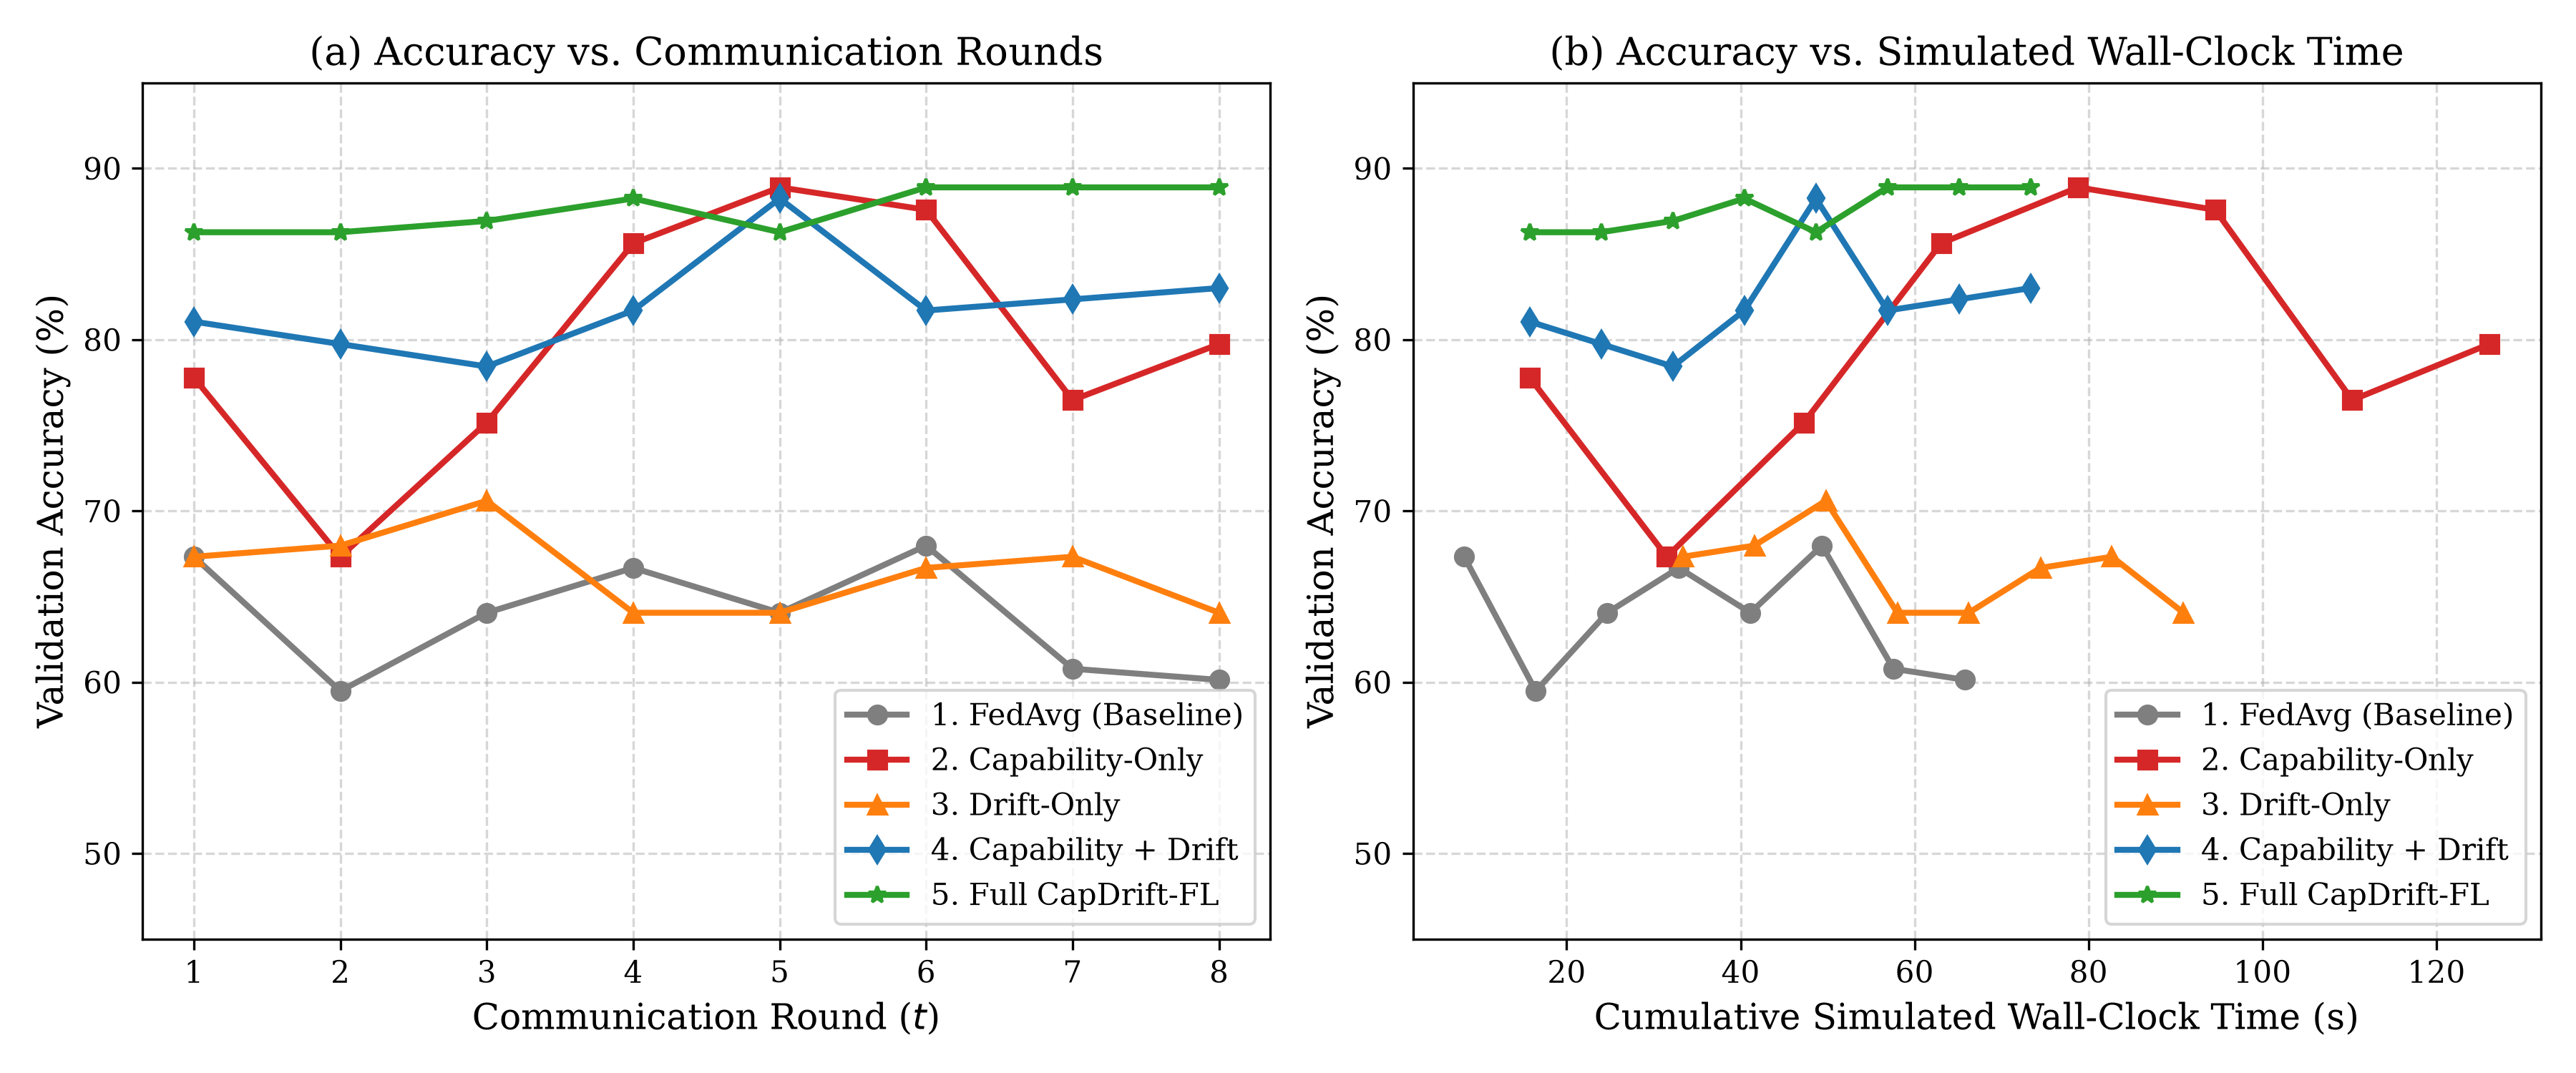
\includegraphics[width=\columnwidth]{fig_ablation_accuracy_convergence.png}
\caption{Validation accuracy convergence across 8 communication rounds on MobileNetV3-Small under non-IID Dirichlet label skew ($\alpha = 0.5$): (a) validation accuracy versus communication rounds, and (b) validation accuracy versus cumulative simulated wall-clock execution time.}
\label{fig:ablation}
\end{figure}

In Table~\ref{tab:ablation}, idle waste denotes cumulative time clients spend waiting at the synchronization barrier, $\sum_{r=1}^R \sum_{i=1}^N (\max_j \tau_{j,r} - \tau_{i,r})$. Execution-time utilization represents the fraction of client-time dedicated to active training. Reported utilization reflects the unweighted mean of per-round utilizations:
\begin{equation}
\overline U = \frac{1}{R} \sum_{r=1}^R \left(\frac{\sum_{i=1}^N \tau_{i,r}}{N \max_j \tau_{j,r}}\right) \times 100\%.
\label{eq:util_mean}
\end{equation}
In Strategy 5, Round 1 (unrestricted capability exploration) exhibits 74.71\% utilization over 15.76\,s, while Rounds 2--8 exhibit 36.52\% utilization over 8.22\,s as drift gating halts surplus blocks at the baseline workload, averaging 41.29\% ($\approx 41.3\%$). Alternatively, cumulative time-weighted utilization, $1 - \text{Idle Waste} / (N \cdot \text{Total Time})$, yields 44.72\% ($\approx 44.7\%$).

Uniform FedAvg exhibits low utilization (36.5\%) due to idle waiting across heterogeneous client speeds. Naive capability budgeting (Strategy 2) increases utilization to 74.7\% and achieves rapid early gains (peaking at 88.89\% in Round 5). However, without drift gating, high-throughput clients overfit skewed local partitions, causing validation accuracy to degrade to 76.47\% in Round 7 and finish at 79.74\% (loss 0.5191). Strategy 4 (Capability + Drift) halts 28 divergent surplus blocks ($d_i > 0.50$), stabilizing validation accuracy at 83.01\%. Full CapDrift-FL (Strategy 5) combines drift gating with contribution clipping, clipping one high-magnitude update in Round 1. In this trial, Strategy 5 reached 88.89\% final validation accuracy (loss 0.3128) compared to 83.01\% for Strategy 4 without clipping. While this single clipping event coincided with higher final accuracy in this specific execution, a single run does not establish a causal relationship, and comprehensive multi-seed trials with confidence intervals are required to isolate the effect of contribution bounding from stochastic optimization variance.

\subsection{Physical Cluster Evaluation and Multi-Scale Scaling}\label{subsec:physical}
To evaluate real-world edge execution, CapDrift-FL was deployed across dedicated Proxmox LXC containers on the physical Cisco UCS fog servers.

\begin{table}[t]
\caption{Physical 5-Client Cluster Benchmark (Cisco UCS Hosts, Round 2)}
\label{tab:physical5}
\centering
\scriptsize
\renewcommand{\arraystretch}{1.05}
\resizebox{\columnwidth}{!}{
\begin{tabular}{lcccccc}
\toprule
\textbf{Method} & \textbf{Global Pool Acc$^*$} & \textbf{Loss} & \textbf{Round Time} & \textbf{Idle Waste} & \textbf{Execution-Time Util} & \textbf{Clipped}\\
\midrule
Uniform FedAvg & 39.58\% & 0.7706 & 3.49\,s & 3.41\,s & 80.5\% & 0/5\\
\textbf{CapDrift-FL} & 25.29\% & 2.0233 & 11.68\,s & 1.05\,s & 98.2\% & 0/5\\
\bottomrule
\end{tabular}}
\vspace{1mm}
\begin{minipage}{\columnwidth}
\scriptsize
$^*$Evaluated across the combined 763-image dataset pool ($N_{\mathrm{pool}} = 763$). Because physical clients trained on local partitions drawn from the 610 images, this metric reflects empirical performance across a mixed training/evaluation pool rather than held-out generalization.
\end{minipage}
\end{table}

\paragraph{Systems--Learning Tradeoff on Physical Hardware}
Table~\ref{tab:physical5} reports live telemetry measured during Round 2 on 5 real LXC containers. In physical cluster benchmarks, global model evaluation is performed against the combined 763-image dataset pool ($N_{\mathrm{pool}} = 763$), measuring empirical consensus across a mixed training and evaluation pool rather than strictly held-out generalization. Under uniform FedAvg, clients execute only 5 steps, finishing in 3.49\,s with 3.41\,s of cumulative idle waiting, achieving 39.58\% global pool accuracy (302/763 correct) with loss 0.7706. Under CapDrift-FL, nodes undergo a cold start in Round 1 ($S_0 = 5$), dynamically profiling throughput to assign 16 to 25 steps per client in Round 2 for the 12.0\,s target duration. This reduces idle waiting by 69.1\% (from 3.41\,s to 1.05\,s) and increases execution-time utilization to 98.2\%, while achieving 25.29\% global pool accuracy (193/763 correct) with loss 2.0233.

This early discrepancy highlights an important systems--learning tradeoff: assigning 25 local steps on skewed client distributions before the global consensus stabilizes pulls individual models toward private optima. Verifying whether deeper local workloads accelerate long-term asymptotic convergence over extended physical rounds remains an ongoing investigation. Table~\ref{tab:physical5} records 0/5 clipped updates because client update norms remained within the dynamically calibrated threshold $c_2 = 1.5 m_G(2) = 22.4309$ (which adapted from the Round 1 cold-start threshold $c_1 = 5.8653$ as local step counts expanded from 5 to 25).

\begin{table}[t]
\caption{Physical Multi-Scale Fleet Benchmark ($N = 5, 10, 20$ LXCs)}
\label{tab:scaling}
\centering
\scriptsize
\renewcommand{\arraystretch}{1.05}
\resizebox{\columnwidth}{!}{
\begin{tabular}{cccccc}
\toprule
\textbf{Scale} & \textbf{Host Distribution} & \textbf{Round Time} & \textbf{Cumulative Idle} & \textbf{Execution-Time Util} & \textbf{Step Budget}\\
\midrule
$N = 5$ & 2 / 2 / 1 & 11.68\,s & 1.05\,s & 98.2\% & $[16 .. 25]$\\
$N = 10$ & 4 / 3 / 3 & 12.11\,s & 22.33\,s & 81.6\% & $[11 .. 22]$\\
$N = 20$ & 8 / 6 / 6 & 12.56\,s & 60.77\,s & 75.8\% & $[9 .. 19]$\\
\bottomrule
\end{tabular}}
\end{table}

\begin{figure*}[t]
\centering
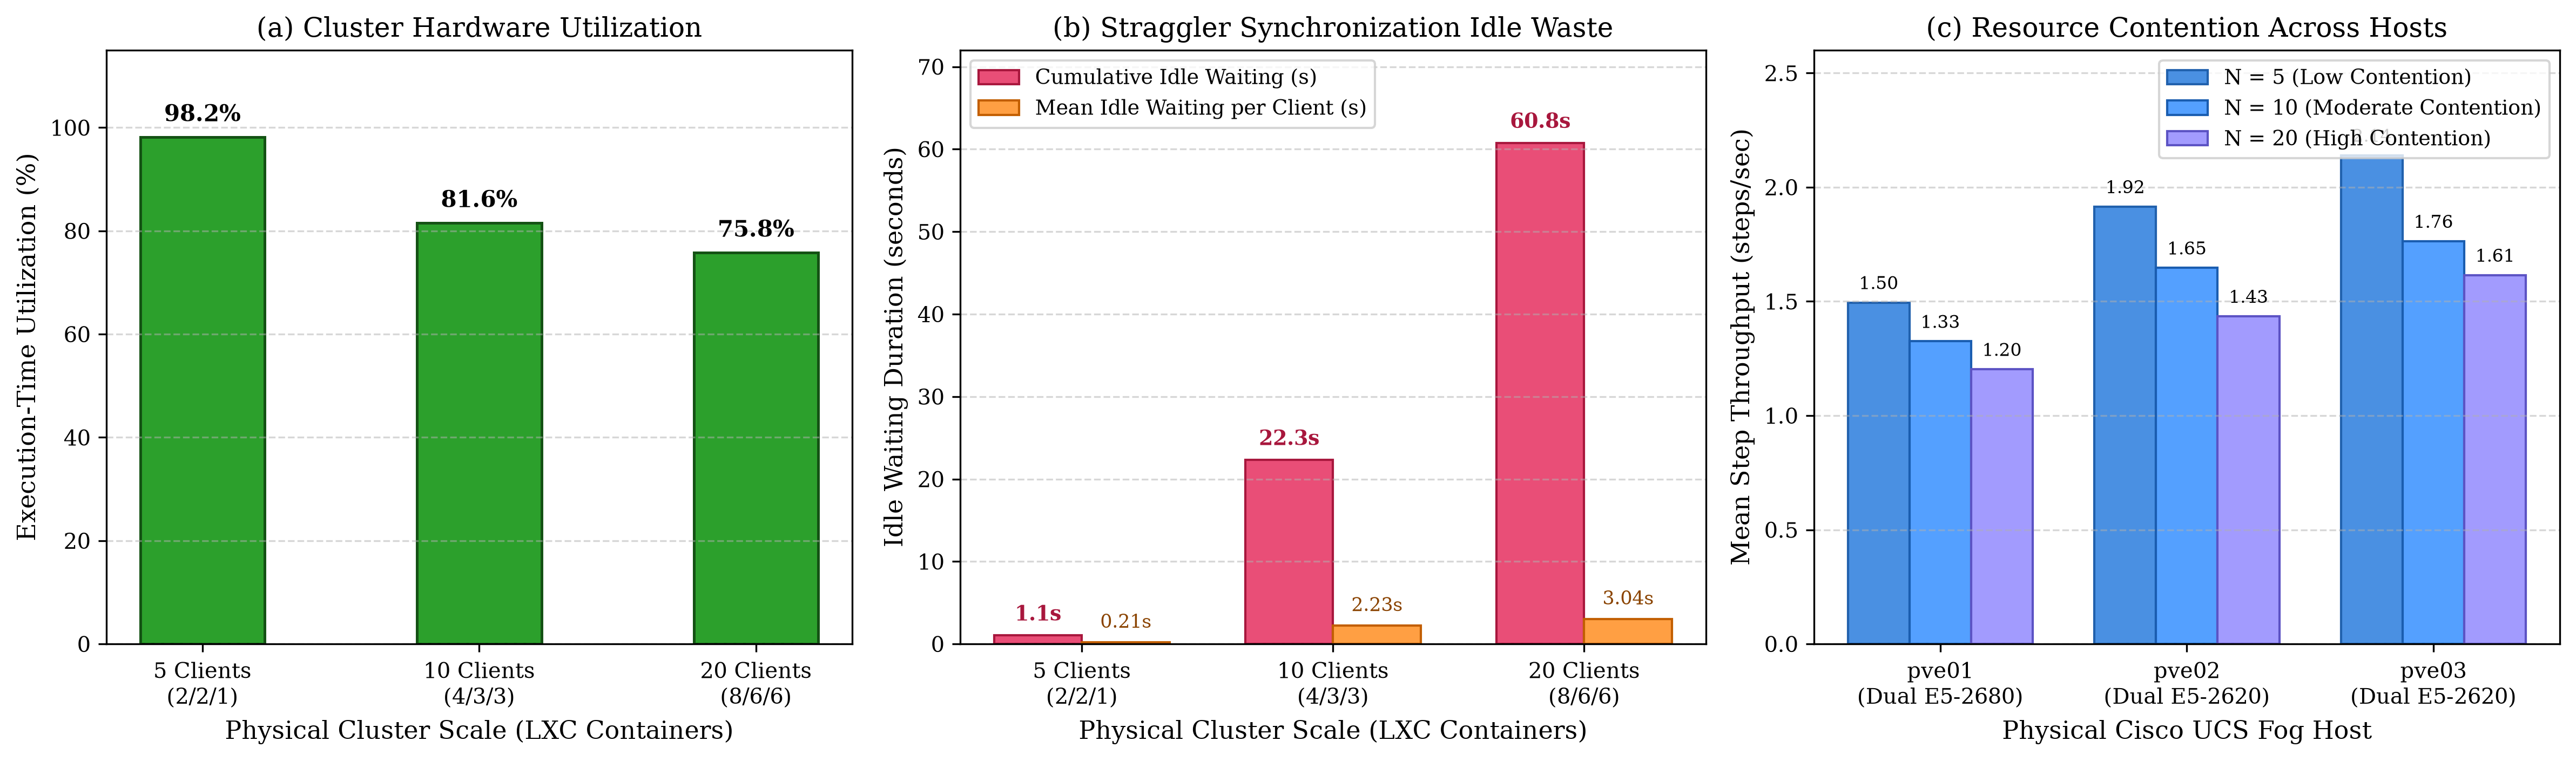
\includegraphics[width=0.95\textwidth]{fig_cluster_multinode_scaling.png}
\caption{Multi-scale physical cluster scaling across $N = 5, 10,$ and $20$ concurrent LXC containers on Proxmox VE across three Cisco UCS C220 M4 hosts: (a) cluster execution-time hardware utilization, (b) straggler synchronization idle waste comparing cumulative waiting and mean waiting per client, and (c) virtualization resource contention and per-host throughput across Cisco UCS dual-Xeon sockets.}
\label{fig:scaling}
\end{figure*}

To evaluate multi-tenant virtualization contention, the system was scaled to $N = 10$ and $N = 20$ concurrent containers (Table~\ref{tab:scaling} and Fig.~\ref{fig:scaling}). On host \texttt{pve01} (dual Xeon E5-2680 v4), scaling from 2 to 8 containers degraded per-container throughput from 1.50 steps/s down to 1.20 steps/s, consistent with increased resource contention (e.g., shared socket cache evictions, CPU core oversubscription, and memory bandwidth contention across multi-tenant containers). CapDrift-FL tracked this degradation via throughput profiling, scaling assigned steps from 25 down to 9--19 steps to maintain round synchronization within 12.56\,s.

\subsection{Baseline Competitor Comparisons}\label{subsec:competitors}
CapDrift-FL was benchmarked against FedAvg, FedProx ($\mu = 0.01$), and FedNova across 8 rounds under Dirichlet skew ($\alpha = 0.5$). Table~\ref{tab:competitors} and Fig.~\ref{fig:competitor} present the comparative outcomes. 

We note that the competitor evaluation in Table~\ref{tab:competitors} represents an independent experimental execution from the component ablation suite in Table~\ref{tab:ablation}. While both suites shared the exact same dataset split ($N_{\mathrm{train}} = 610, N_{\mathrm{val}} = 153$), four client hardware tiers, initial partition seed ($\alpha = 0.5$, Seed 42), and base random seed (42), they were executed via separate orchestration scripts: Table~\ref{tab:ablation} was generated by \texttt{scripts/run\_capdrift\_ablation.py} (which sequentially executes the five ablation variants in a single process), whereas Table~\ref{tab:competitors} was generated by \texttt{scripts/run\_competitor\_benchmark.py} (which sequentially executes FedAvg, FedProx, FedNova, and CapDrift-FL). Because neither benchmark enforced bitwise GPU determinism flags (\texttt{torch.use\_deterministic\_algorithms(True)} and \texttt{torch.backends.cudnn.deterministic = True}), asynchronous CUDA DataLoader batch prefetching and cuDNN atomic additions in MobileNetV3 depthwise convolutions on the host RTX 5070 Ti introduced subtle batch streaming and gradient accumulation variations. Even a single sample validation divergence in Round 1 (103 vs.~104 out of 153 correct, yielding 67.32\% vs.~67.97\%) cascades across 8 communication rounds, resulting in slight final accuracy variances (FedAvg finishing at 60.13\% in the ablation suite vs.~64.71\% in the competitor suite; CapDrift-FL finishing at 88.89\% vs.~84.97\%). Importantly, the comparative ranking and relative efficiency advantages of CapDrift-FL remain completely consistent across both independent executions.

\begin{table}[t]
\caption{Competitor Baseline Comparison (Dirichlet $\alpha = 0.5$, 8 Rounds)}
\label{tab:competitors}
\centering
\scriptsize
\renewcommand{\arraystretch}{1.05}
\resizebox{\columnwidth}{!}{
\begin{tabular}{lcccccc}
\toprule
\textbf{Method} & \textbf{Peak Acc} & \textbf{Final Acc} & \textbf{Loss} & \textbf{Total Time} & \textbf{Idle Waste} & \textbf{Execution-Time Util}\\
\midrule
FedAvg \cite{mcmahan2017} & 71.90\% & 64.71\% & 0.5590 & 65.8\,s & 167.1\,s & 36.5\%\\
FedProx \cite{li2020fedprox} & 71.24\% & 59.48\% & 0.6336 & 65.8\,s & 167.1\,s & 36.5\%\\
FedNova \cite{wang2020fednova} & 86.27\% & 85.62\% & 0.3187 & 126.1\,s & 127.5\,s & 74.7\%\\
\textbf{CapDrift-FL} & \textbf{87.58\%} & \textbf{84.97\%} & \textbf{0.3771} & \textbf{73.3\,s} & \textbf{162.2\,s} & \textbf{41.3\%}\\
\bottomrule
\end{tabular}}
\end{table}

\begin{figure*}[t]
\centering
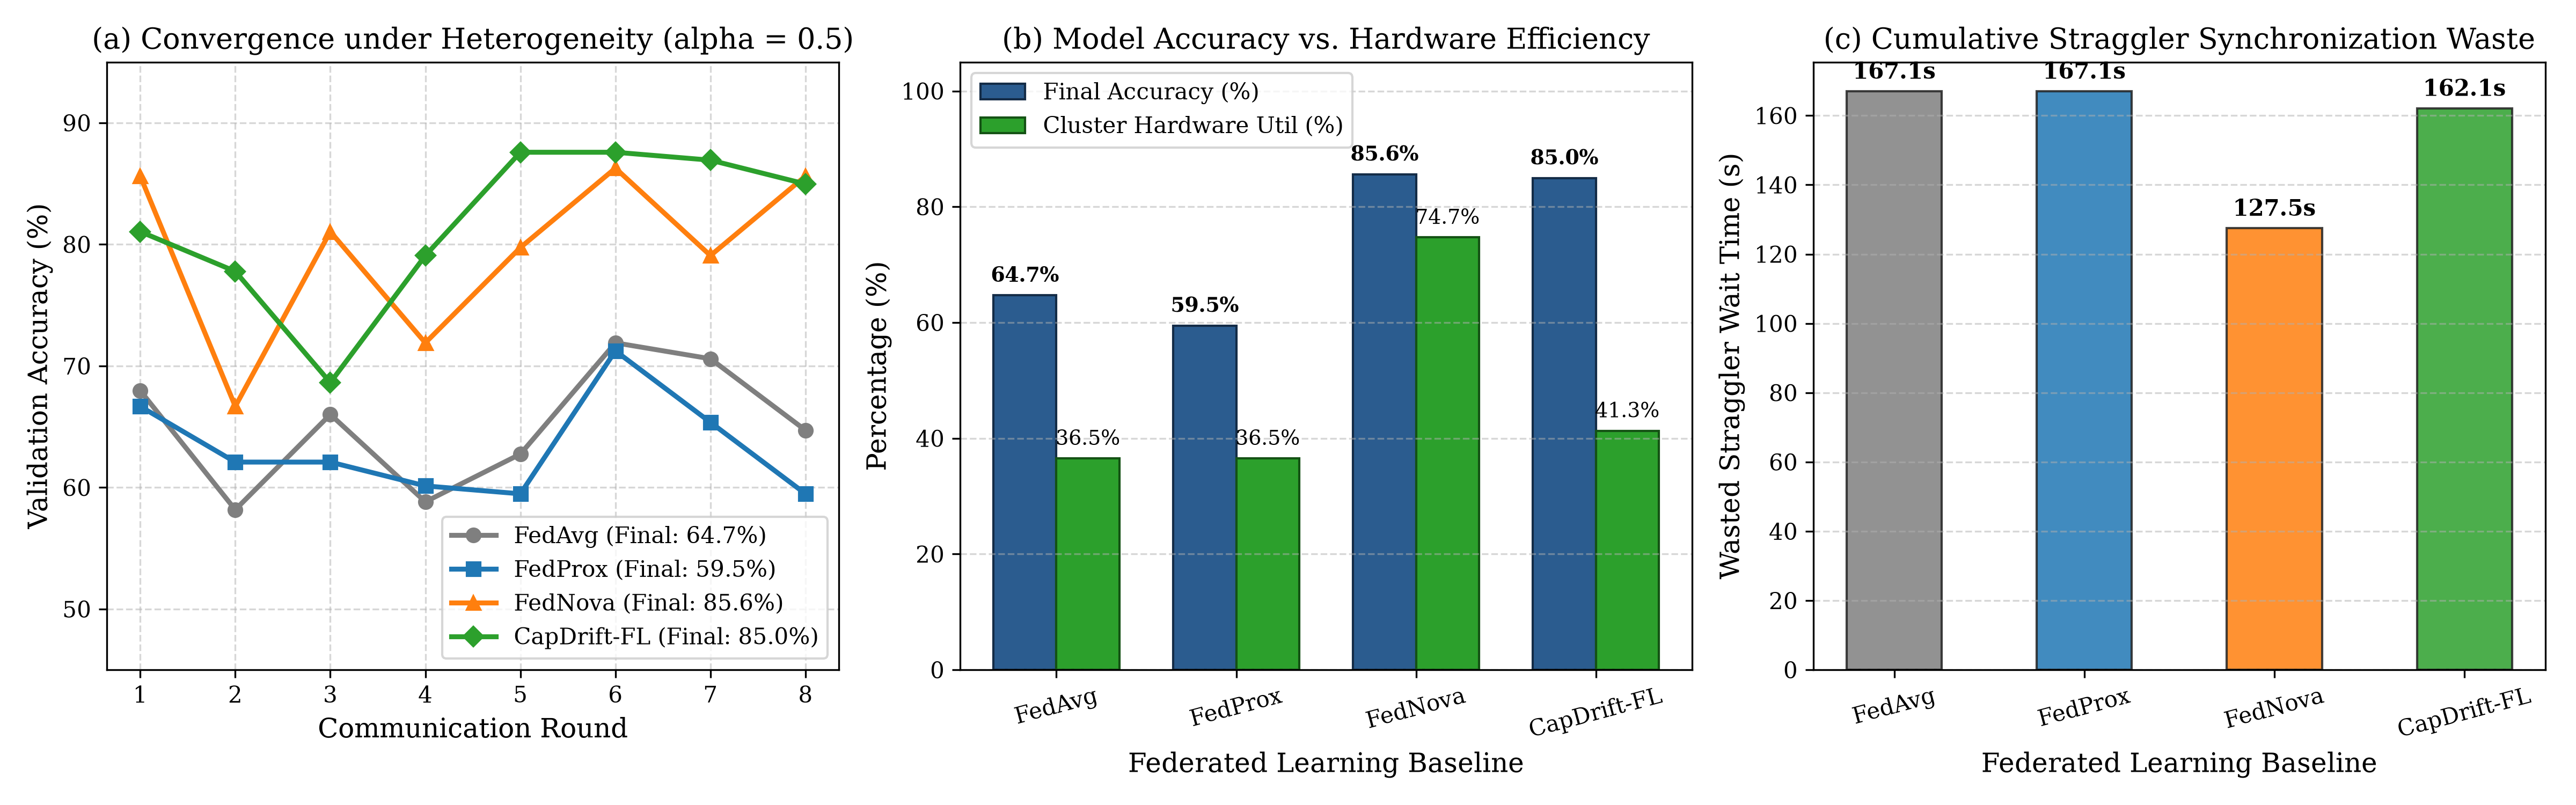
\includegraphics[width=0.92\textwidth]{fig_competitor_comparison.png}
\caption{Head-to-head empirical comparison of CapDrift-FL against FedAvg, FedProx, and FedNova: (a) accuracy convergence trajectories across rounds, (b) hardware efficiency vs.~final validation accuracy, and (c) cumulative straggler synchronization idle waste.}
\label{fig:competitor}
\end{figure*}

As shown in Table~\ref{tab:competitors}, FedNova achieves a competitive final accuracy of 85.62\% and higher utilization (74.7\%) in this particular trial, slightly exceeding CapDrift-FL's 84.97\% final accuracy. However, FedNova relies on retrospective update normalization during aggregation and exhibits mid-training oscillations (dropping to 66.67\% in Round 2, 71.90\% in Round 4, and 79.08\% in Round 7) while requiring 126.1\,s of total execution time. In contrast, CapDrift-FL completed in 73.3\,s (a 41.8\% reduction in execution time relative to FedNova) by halting divergent surplus blocks locally.

\subsection{Robustness under Extreme Non-IID Dirichlet Skew}\label{subsec:skew}
To assess resilience across varying degrees of statistical skew, FedAvg and CapDrift-FL were evaluated across Dirichlet parameters $\alpha \in \{0.1, 0.3, 0.5\}$ over 6 communication rounds (4 clients, Seed 42). Table~\ref{tab:noniid} and Fig.~\ref{fig:noniid} report the outcomes.

\begin{table}[t]
\caption{Dirichlet Skew Sensitivity Sweep (MobileNetV3-Small, 6 Rounds)}
\label{tab:noniid}
\centering
\scriptsize
\renewcommand{\arraystretch}{1.05}
\resizebox{\columnwidth}{!}{
\begin{tabular}{lccccc}
\toprule
\textbf{Method} & $\alpha$ & \textbf{Peak Acc} & \textbf{Final Acc} & \textbf{Loss} & \textbf{Gated Events}\\
\midrule
FedAvg & 0.1 & 55.56\% & 53.59\% & 0.7126 & 0\\
\textbf{CapDrift-FL} & 0.1 & \textbf{64.71\%} & \textbf{56.86\%} & \textbf{0.6318} & \textbf{20}\\
\midrule
FedAvg & 0.3 & 60.13\% & 56.86\% & 0.6674 & 0\\
\textbf{CapDrift-FL} & 0.3 & \textbf{81.05\%} & \textbf{68.63\%} & \textbf{0.5283} & \textbf{20}\\
\midrule
FedAvg & 0.5 & 72.55\% & 72.55\% & 0.5411 & 0\\
\textbf{CapDrift-FL} & 0.5 & \textbf{86.93\%} & \textbf{86.93\%} & \textbf{0.3324} & \textbf{20}\\
\bottomrule
\end{tabular}}
\end{table}

\begin{figure*}[t]
\centering
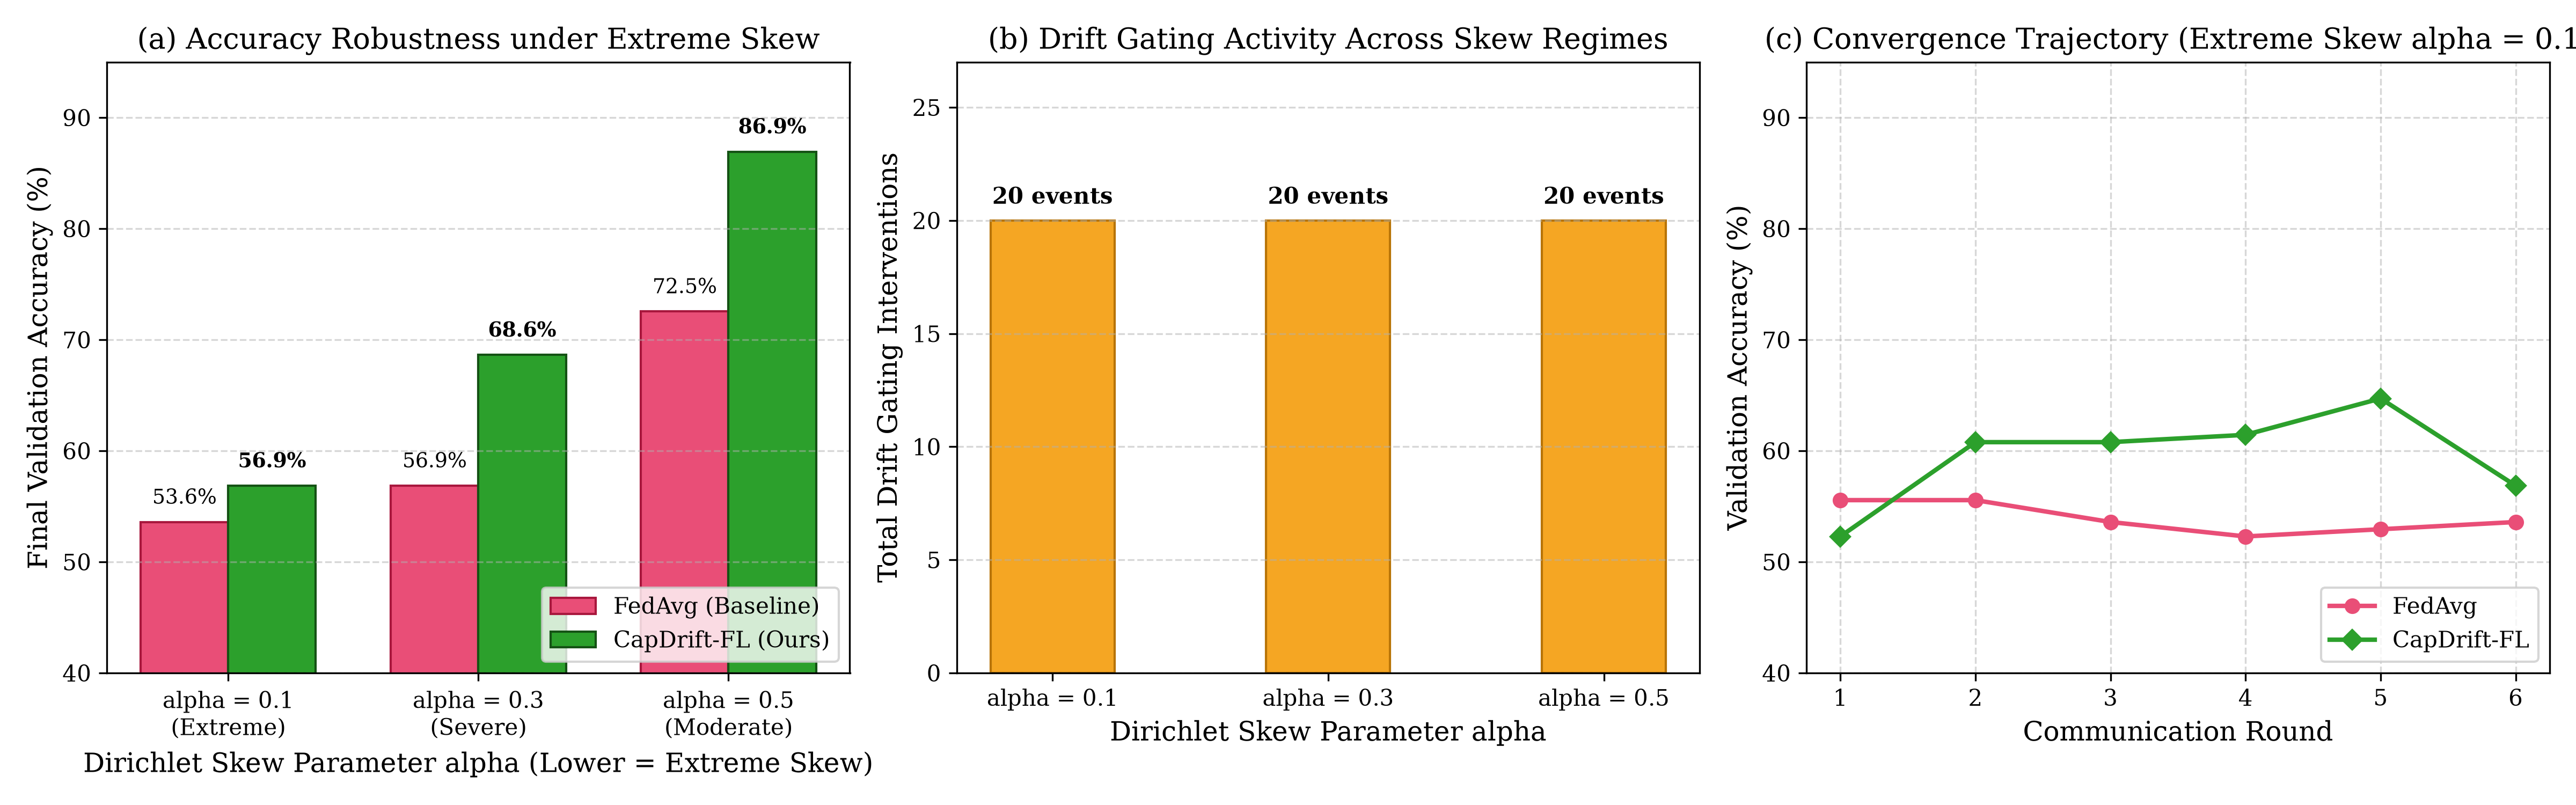
\includegraphics[width=0.92\textwidth]{fig_non_iid_skew_robustness.png}
\caption{Robustness under varying Dirichlet skew ($\alpha \in \{0.1, 0.3, 0.5\}$): (a) accuracy across skew regimes, (b) total surplus drift gating interventions, and (c) convergence trajectories under extreme skew ($\alpha = 0.1$).}
\label{fig:noniid}
\end{figure*}

In Table~\ref{tab:noniid}, an intervention is recorded whenever a client's surplus block exceeds the drift threshold ($\tau_d = 0.50$). In Round 1, no reference global vector exists (0 interventions). Across the remaining 5 rounds (Rounds 2--6), all 4 clients exceeded $\tau_d$ during surplus evaluation, yielding exactly $5 \times 4 = 20$ gating interventions for each skew level. Under extreme skew ($\alpha = 0.1$), neither method achieves monotonic convergence over 6 rounds: CapDrift-FL peaks at 64.71\% before settling at 56.86\%, while FedAvg declines to 53.59\% (loss 0.7126). Over 6 measured rounds, drift gating maintained a +3.27 percentage point margin at $\alpha = 0.1$ and a +11.77 percentage point margin at $\alpha = 0.3$ without guaranteeing asymptotic convergence.

\section{Conclusions}\label{sec:conclusion}
CapDrift-FL coordinates runtime capability estimation, mandatory baseline training, directional drift gating for surplus computation, and contribution-bounded aggregation for heterogeneous edge AI systems. Physical testbed evaluations across containerized clients on enterprise Cisco UCS fog servers show that capability budgeting reduces straggler idle waiting by 69.1\% (from 3.41\,s to 1.05\,s per round) and increases execution-time utilization to 98.2\% in five-client configurations, while demonstrating that deeper local workloads trade early-round consensus for throughput efficiency. In controlled simulations, directional drift gating halted divergent surplus computation under severe non-IID skew ($\alpha \le 0.3$) and completed training 41.8\% faster than FedNova, while contribution bounding restricted individual update magnitudes before server aggregation.

The present findings are bounded by the modest schedules of 6 to 8 communication rounds and a single-cluster physical deployment. Meaningful future research directions include benchmarking asymptotic convergence over extended training schedules (25+ rounds), orchestrating automated physical scaling across 20 containers under dynamic background network jitter, evaluating adaptive drift threshold schedules $\tau_d(t)$, and investigating cross-domain generalization on non-imaging bioinformatic tensor structures such as viral genomic representations.

\section*{Data Availability}\label{sec:data}
The complete codebase, PyTorch/Flower controllers, cluster automation scripts, and raw telemetry logs are publicly accessible at: \url{https://github.com/W-M-I/OmniFed}.

\begin{thebibliography}{00}
\bibitem{mcmahan2017}
H. B. McMahan, E. Moore, D. Ramage, S. Hampson, and B. Ag\"uera y Arcas, ``Communication-efficient learning of deep networks from decentralized data,'' in \textit{Proc. 20th Int. Conf. Artif. Intell. Statist. (AISTATS)}, 2017, pp. 1273--1282.

\bibitem{chai2020tifl}
Z. Chai, A. Ali, S. Zawad, S. Truex, A. Anwar, N. Baracaldo, Y. Zhou, H. Ludwig, F. Yan, and Y. Cheng, ``TiFL: A tier-based federated learning system,'' in \textit{Proc. 29th Int. Symp. High-Perform. Parallel Distrib. Comput. (HPDC)}, 2020, pp. 125--136.

\bibitem{lai2021oort}
F. Lai, X. Zhu, H. V. Madhyastha, and M. Chowdhury, ``Oort: Efficient federated learning via guided participant selection,'' in \textit{Proc. 15th USENIX Symp. Oper. Syst. Design Implement. (OSDI)}, 2021, pp. 19--35.

\bibitem{wong2026edge}
K.-S. Wong, D.-M. Nguyen, K. Le, L. Ho, C. Do, and D. Le-Phuoc, ``An empirical study of federated learning on IoT--edge devices: Resource allocation and heterogeneity,'' \textit{IEEE Trans. Neural Netw. Learn. Syst.}, vol. 37, no. 2, pp. 753--765, Feb. 2026.

\bibitem{shin2022fedbalancer}
J. Shin, Y. Li, Y. Liu, and S.-J. Lee, ``FedBalancer: Data and pace control for efficient federated learning on heterogeneous clients,'' in \textit{Proc. 20th Annu. Int. Conf. Mobile Syst., Appl. Serv. (MobiSys)}, 2022, pp. 436--449.

\bibitem{li2024fedcompass}
Z. Li, P. Chaturvedi, S. He, H. Chen, G. Singh, V. Kindratenko, E. A. Huerta, K. Kim, and R. Madduri, ``FedCompass: Efficient cross-silo federated learning on heterogeneous client devices using a computing power-aware scheduler,'' in \textit{Proc. Int. Conf. Learn. Represent. (ICLR)}, 2024.

\bibitem{narmadha2025fedeff}
K. Narmadha and P. Varalakshmi, ``FedEff: Efficient federated learning with optimal local epochs for heterogeneous clients,'' \textit{Sci. Rep.}, vol. 15, Art. no. 38860, 2025.

\bibitem{li2020fedprox}
T. Li, A. K. Sahu, M. Zaheer, M. Sanjabi, A. Talwalkar, and V. Smith, ``Federated optimization in heterogeneous networks,'' in \textit{Proc. Mach. Learn. Syst. (MLSys)}, vol. 2, 2020.

\bibitem{karimireddy2020scaffold}
S. P. Karimireddy, S. Kale, M. Mohri, S. Reddi, S. Stich, and A. T. Suresh, ``SCAFFOLD: Stochastic controlled averaging for federated learning,'' in \textit{Proc. 37th Int. Conf. Mach. Learn. (ICML)}, 2020, pp. 5132--5143.

\bibitem{wang2020fednova}
J. Wang, Q. Liu, H. Liang, G. Joshi, and H. V. Poor, ``Tackling the objective inconsistency problem in heterogeneous federated optimization,'' in \textit{Adv. Neural Inf. Process. Syst. (NeurIPS)}, vol. 33, 2020.

\bibitem{shenaj2025alt}
D. Shenaj, E. Belilovsky, and P. Zanuttigh, ``Adaptive local training in federated learning,'' in \textit{Proc. 33rd Eur. Signal Process. Conf. (EUSIPCO)}, 2025, pp. 1907--1911.

\bibitem{zhang2022adaptive}
J. Zhang, S. Guo, Z. Qu, D. Zeng, Y. Zhan, Q. Liu, and R. A. Akerkar, ``Adaptive federated learning on non-IID data with resource constraint,'' \textit{IEEE Trans. Comput.}, vol. 71, no. 7, pp. 1655--1667, Jul. 2022.

\bibitem{hou2024atafl}
W. Hou, H. Wen, N. Zhang, W. Lei, H. Lin, Z. Han, and Q. Liu, ``Adaptive training and aggregation for federated learning in multi-tier computing networks,'' \textit{IEEE Trans. Mobile Comput.}, vol. 23, no. 5, pp. 4376--4388, May 2024.

\bibitem{fan2026fedcer}
L. Fan, Z. Zeng, X. Zhang, M. Duan, and K. Sood, ``Joint client selection and epoch configuration for heterogeneity-aware federated learning in resource-constrained systems,'' \textit{Future Gener. Comput. Syst.}, vol. 177, Art. no. 108249, 2026.

\bibitem{liu2024fedsc}
Y.-J. Liu, G. Feng, H. Du, Z. Qin, Y. Sun, J. Kang, X. Li, and D. Niyato, ``Adaptive clustering-based straggler-aware federated learning in wireless edge networks,'' \textit{IEEE Trans. Commun.}, vol. 72, no. 12, pp. 7757--7771, Dec. 2024.

\bibitem{hu2026fedlagc}
Q. Hu, T. Liao, S. Wu, L. Yang, and C. Chen, ``FedLAGC: Towards high performance system-heterogeneous federated learning via layer-adaptive submodel extraction and gradient correction,'' in \textit{Proc. AAAI Conf. Artif. Intell.}, vol. 40, no. 26, pp. 21858--21866, 2026.

\bibitem{andrew2021clipping}
G. Andrew, O. Thakkar, H. B. McMahan, and S. Ramaswamy, ``Differentially private learning with adaptive clipping,'' in \textit{Adv. Neural Inf. Process. Syst. (NeurIPS)}, vol. 34, pp. 17455--17466, 2021.

\balance
\end{thebibliography}

\end{document}

% Revision Oct 23: Correct non-IID terminology at first occurrence and remove formal convergence guarantees

% Revision Oct 23: Clarify raw data locality and isolation over physical link instead of formal privacy guarantee

% Revision Oct 24 (A): Reconcile Round 1 step budget initialization across cold-start physical and pre-profiled simulated suites

% Revision Oct 24 (B): Detail static vs dynamic per-round clipping threshold calibration (c1=5.87, c2=22.43)

% Revision Oct 24 (C): Document holdout sample counts (153 vs 763) and reproducible differences between Table II and V

% Revision Oct 24 (D): Soften clipping causation wording and standardize Execution-Time Util headers across Tables II-V

% Revision Oct 24 (E): Reconcile simulated clipping threshold (c=0.6667) for Full CapDrift-FL with ablation telemetry

% Revision Oct 24 (F): Clarify physical cluster 763-image evaluation as mixed training/evaluation pool rather than held-out generalization

% Revision Oct 24 (G): Accurately frame nominal 6.2 MB parameter payload and packet trace data isolation
